\documentclass{article}
\usepackage{graphicx}
\usepackage{amsmath}
\usepackage{hyperref}
\usepackage{float}
\usepackage{xcolor}
\usepackage{enumitem}

\begin{document}

\title{Solutions to hw8 homework on Convex Optimization https://web.stanford.edu/class/ee364a/homework.html}
\author{Andrei Keino}
\maketitle

\section*{9.8}

\textit{Steepest descent method in l$_{\infty}$-norm.} Explain how to find a steepest descent direction
in the l$_{\infty}$-norm, and give a simple interpretation.

\textbf{Solution}. 

The normalized steepest descent direction is given by
$$
\Delta x_{nsd} = - sign(\nabla f(x))
$$

where the sign is taken componentwise. Interpretation: If the partial derivative with
respect to $x_k$ is positive we take a step that reduces $x_k$; if it is positive, we take a step
that increases $x_k.$ \\
The unnormalized steepest descent direction is given by
$$
\Delta x_{sd} = - ||f(x)||_1 sign(\nabla f(x))
$$


\section*{10.1}

\textit{Nonsingularity of the KKT matrix.} Consider the KKT matrix

$$
\begin{bmatrix} 
	P & A^T \\
	A & 0\\
\end{bmatrix}
$$
where $P \in S^n_+,$ $A \in R^{p \times n},$ and rank 
$A = p < n.$

(a) Show that each of the following statements is equivalent to nonsingularity of the
KKT matrix.

\begin{enumerate}
	\item $\mathcal{N}(P) \cap \mathcal{N}(A) = \{0\}. $ 
	\item $Ax = 0, \; x \ne 0 \Rightarrow x^T P x \ne 0. $ 
	\item $F^T P F \succ 0$ where 
	$F \in R^{n \times (n - p)}$ is a matrix for which
	$\mathcal{R}(F) = \mathcal{N}(A).$
	\item $P + A^T Q A \succ 0$ for some $Q \succeq 0.$
\end{enumerate}

\textbf{Solution.} \\

\begin{enumerate}[label=\alph*)]
\item 
\begin{itemize}
    \item \textit{Conditions 1 and 2.}
    If $x \in \mathcal{N}(P) \cap \mathcal{N}(A),$ 
    $x \ne 0,$ then $Ax = 0,$ $x \ne 0$ but $x^T P x = 0,$
    contradicting the second statement. Conversely, suppose the second statement fails to hold, 
    \textit{i.e.}, there is an $x$ with $Ax = 0,$
    $x \ne 0,$ but $x^T P x = 0.$ Since $P \succeq 0$ 
    we conclude $Px = 0,$ \textit{i.e.},
    $x \in \mathcal{N}(P),$ which
    contradicts the first statement.
    	
	\item \textit{Conditions 2 and 3.}
	If $Ax = 0, \; x \ne 0,$ 
	then x must have the form
	$x = Fz$ where $z \ne 0,$
	because $rank(F) = n - p.$ Then we have
	$x^T P x = z^T F^T P F z > 0.$
	
	\item \textit{Conditions 2 and 4.} 
	If the second condition holds then 
	$$
	x^T(P + A^TA)x = x^TPx + ||Ax||_2^2 > 0
	$$
	for all nonzero x, so the last statement holds with
	$Q = I.$ It the last statement holds for some 
	$Q \succeq 0$ then
	$$
	x^T(P + A^TQA)x = x^TPx + x^T A^T Q A x > 0	
	$$
	for all nonzero x. Therefore if 
	$Ax = 0$ and $x \ne 0$ we must have $x^TPx > 0.$ \\
	Now let us show that the four statements are equivalent to nonsingularity of the
	KKT matrix. First suppose that $x$ satisfies 
	$Ax = 0,$ $Px = 0$ and $x \ne 0.$ Then 
	$$
	\begin{bmatrix} 
		P & A^T \\
		A & 0\\
	\end{bmatrix}
	\begin{bmatrix} 
	x\\
	0\\
	\end{bmatrix} = 0
	$$
which shows that the KKT matrix is singular.\\
Now suppose the KKT matrix is singular, i.e., there are $x, z,$ not both zero, such that	
	$$
\begin{bmatrix} 
	P & A^T \\
	A & 0\\
\end{bmatrix}
\begin{bmatrix} 
	x\\
	z\\
\end{bmatrix} = 0
$$
This means that $Px + A^Tz = 0$ and $Ax = 0,$ so multiplying the first equation by $x^T$ on the left 
we get $x^TPx + x^TA^Tz = 0.$ Using $Ax = 0,$ we get 
$x^T P x = 0,$ so we have $Px = 0$ (using $P \succeq 0$).
This contradicts (a) unless we have $x = 0.$ In this case we must have $z \ne 0.$ But then $A^Tz = 0$ contradicts 
$rank(A) = p.$

\end{itemize}
	
\item From part (a) $P + A^TA \succ 0.$ Therefore there exists a nonsingular matrix $R \in R^{n \times n}$ such that
$$
R^T(P + A^TA)R = I
$$
Let $AR = U \Sigma V_1^T$ be the singular value decomposition of $AR$, with $U \in R^{p \times p},$
$\Sigma = diag(\sigma_1, \dots, \sigma_p) \in R^{p \times p}$ and $V_1 \in R{n \times p}.$ Let $V_2 \in R^{n \times (n - p)}$ be such that 
$$
V = [V_1 \quad V_2] 
$$
is orthogonal, and define
$$
S = [\Sigma \quad 0] \in R^{p \times n}.
$$

We have $AR = U \Sigma V^T,$ so
$$
V^TR^T(P + A^TA)RV = V^TR^TPRV + S^TS = I
$$
Therefore $V^TR^TPRV = I - S^TS$ is diagonal. We denote this matrix by $\Lambda:$

$$
\Lambda = V^TR^TPRV = 
\mathbf{diag}(1 - \sigma_1^2, \dots, 1 - \sigma_p^2, 1, \dots, 1).
$$

applying the congruence transformation to the KKT matrix gives 
$$
\begin{bmatrix} 
	V^TR^T & 0 \\
	0 & U^T\\
\end{bmatrix}
\begin{bmatrix} 
	P & A^T \\
	0 & A\\
\end{bmatrix}
\begin{bmatrix} 
	VR & 0 \\
	0 & U\\
\end{bmatrix} = 
\begin{bmatrix} 
	\Lambda & S^T \\
	S^T & 0\\
\end{bmatrix}
$$

and the inertia of the KKT matrix is equal to the inertia of the matrix on the right.
Applying a permutation to the matrix on the right gives a block diagonal matrix with $n$ diagonal blocks
$$
\begin{bmatrix} 
	\lambda_i & \sigma_i \\
	\sigma_i & 0\\
\end{bmatrix}, \quad i = 1, \dots, p
\quad \lambda_i = 1, \quad i = p + 1, \dots, n.
$$

The eigenvalues of the $2 \times 2$ -blocks are:
$$
\frac{\lambda_i \pm \sqrt{\lambda _i ^2 + 4 \sigma _i ^2}}{2}
$$
i.e., one eigenvalue is positive and one is negative. We conclude that there are 
$p + (n - p) = n$ 
positive eigenvalues and 
$p$ negative eigenvalues.

\end{enumerate}

\section*{11.13} 
\textit{Self-concordance and negative entropy.}
\begin{enumerate}[label=(\alph*)]
\item Show that the negative entropy function 
$x log(x)$ (on $R_{++}$) is not self-concordant.
\item Show that for any $t > 0,$ $t x log(x) - log(x)$ 
is self-concordant (on $R_{++}$).
\end{enumerate}

{\bf Solution}\\

\begin{enumerate}[label=(\alph*)]
	\item Consider the function 
	$f(x) = x log(x).$
	$$
	f'(x) = log(x) + 1; \quad
	f''(x) = 1/x; \quad
	f'''(x) = - 1/x^2
	$$
	Thus 
	$$
	\frac{|f'''(x)|}{(f''(x)^{3/2})} = 1/x^{1/2}
	$$
	and this function is not bounded on $R_{++}.$ 
	So, the negative entropy function is not self-concordant.
	
	\item Consider the function 
	$g(x) = t x log(x) - log(x).$ 
	$$
	g'(x) = - 1/x + t + t log(x) \quad
	g''(x) = 1/x^2 + t/x \quad
	g'''(x) = - 2 / x^3 - t / x^2
	$$
Then
$$
\psi(x) = \frac{|f'''(x)|}{(f''(x)^{3/2})} = 
\frac{2 / x^3 + t / x^2}{(1/x^2 + t/x)^{3/2}} =
\frac{2 + t x}{(1 + tx)^{3/2}}
$$	
We have:
$$
\psi(0) = 2, \quad \psi(\infty) = 1
$$
and 
$$
\frac{d \psi}{d(tx)} = 
\frac{(1 + tx)^{3/2} - 3/2 (1 + tx)^{1/2}(2 + tx)}{(1 +tx)^{3}}
= - \frac{2 + tx / 2}{(1 +tx)^{5/2}} < 0 \; \forall \; t > 0, \; x > 0 
$$
It means that 
function $\psi(tx)$ monotonically decreases on $R_{++}$ from $2$ to $1,$ for any $t > 0,$ so we are done. 

\end{enumerate}

\section*{Additional exercises} 

In the following three exercises, you will implement a barrier method for solving the standard
form LP
\begin{align*}
	&\text{minimize } && c^T x \\
	&\text{subject to} && Ax = b, \quad x \succeq 0,\\
\end{align*}
with variable $x \in R^n,$ where $A \in R^{m \ times n},$ with 
$m < n.$ Throughout this exercise we will
assume that $A$ is full rank, and the sublevel sets 
$\{x| \; Ax = b, \; x \succeq 0 \; c^T x < \gamma\}$ are all
bounded. (If this is not the case, the centering problem is unbounded below.)

1. Centering step. Implement Newton’s method for solving the centering problem
\begin{align*}
	&\text{minimize } && c^T x - \sum_{i = 1}^n log(x_i)\\
	&\text{subject to} && Ax = b,\\
\end{align*}
with variable $x$, given a strictly feasible starting point $x_0.$\\

Your code should accept $A, b, c,$ and $x_0$, and return $x^*,$ the primal optimal point, $\nu^*,$
a dual optimal point, and the number of Newton steps executed.\\

Use the block elimination method to compute the Newton step. (You can also compute the Newton step via the KKT system, and compare the result to the Newton step
computed via block elimination. The two steps should be close, but if any $x_i$ is very
small, you might get a warning about the condition number of the KKT matrix.)\\

Plot $\lambda^2 / 2$ versus iteration $k$, for various problem data and initial points, to verify that
your implementation gives asymptotic quadratic convergence. As stopping criterion,
you can use $\lambda^2 / 2 < 10^{-6}.$ Experiment with varying the algorithm parameters $\alpha$ and $beta$,
observing the effect on the total number of Newton steps required, for a fixed problem
instance. Check that your computed $x*$ and $\nu^*$ (nearly) satisfy the KKT conditions.\\

To generate some random problem data (i.e., $A, b, c, x_0$), we recommend the following
approach. First, generate $A$ randomly. (You might want to check that it has full rank.)
Then generate a random positive vector $x_0$, and take $b = Ax_0.$ (This ensures that $x0$
is strictly feasible.) The parameter $c$ can be chosen randomly. To be sure the sublevel
sets are bounded, you can add a row to $A$ with all positive elements. If you want to
be able to repeat a run with the same problem data, be sure to set the state for the
uniform and normal random number generators. \\ \\
Here are some hints that may be useful. \\ \\

\begin{itemize}
	\item We recommend computing $\lambda^2$ using the formula 
	$\lambda ^2 = - \Delta x_{nt} \nabla f(x).$. You don’t
	really need $\lambda$ for anything; you can work with $\lambda^2$ instead. (This is important for
	reasons described below.)
	
	\item There can be small numerical errors in the Newton step $- \Delta x_{nt}$ that you compute.
	When $x$ is nearly optimal, the computed value of $\lambda^2$, i.e., $\lambda ^2 = - \Delta x_{nt} \nabla f(x),$ can
	actually be (slightly) negative. If you take the squareroot to get $\lambda$, you’ll get a
	complex number, and you’ll never recover. Moreover, your line search will never
	exit. However, this only happens when $x$ is nearly optimal. So if you exit on the
	condition $\lambda^2 / 2 \leq 10^{-6},$ everything will be fine, even when the computed value of $\lambda ^2$ is negative.
	
	\item For the line search, you must first multiply the step size $t$ by $beta$ until $x + t \Delta x_{nt}$ is
	feasible (i.e., strictly positive). If you don’t, when you evaluate f you’ll be taking
	the logarithm of negative numbers, and you’ll never recover.
\end{itemize}

2. LP solver with strictly feasible starting point. Using the centering code from part (1),
implement a barrier method to solve the standard form LP

\begin{align*}
	&\text{minimize } && c^T x - \sum_{i = 1}^n log(x_i)\\
	&\text{subject to} && Ax = b,\\
\end{align*}

with variable $x \in R^n$, given a strictly feasible starting point $x_0.$ Your LP solver should
take as argument $A, b, c,$ and $x_0,$ and return $x^*.$ \\

You can terminate your barrier method when the duality gap, as
measured by $n/t,$ is smaller then $10^{-3}.$ (If you make
the tolerance much smaller, you might run into
some numerical trouble.) Check your LP solver against the solution found by cvx, for several problem instances.\\

The comments in part (1) on how to generate random data hold here too.\\

Plot the progress of the algorithm, for a problem instance with $n = 500$ and $m = 100,$
showing duality gap (on a log scale) on the vertical axis, versus the cumulative total
number of Newton steps (on a linear scale) on the horizontal axis. \\

Your algorithm should return a $2 \times k$ matrix history, (where $k$ is the total number
of centering steps), whose first row contains the number of Newton steps required
for each centering step, and whose second row shows the duality gap at the end of
each centering step. In order to get a plot that looks like the ones in the book (e.g.,
figure 11.4, page 572), you should use the following code:

\begin{verbatim}
[xx, yy] = stairs(cumsum(history(1,:)),history(2,:));
semilogy(xx,yy);
\end{verbatim}

3. LP solver. Using the code from part (2), implement a general standard form LP
solver, that takes arguments $A, b, c,$ determines (strict) feasibility, and returns an
optimal point if the problem is (strictly) feasible.\\

You will need to implement a phase I method, that determines whether the problem
is strictly feasible, and if so, finds a strictly feasible point, which can then be fed to
the code from part (2). In fact, you can use the code from part (2) to implement the phase I method. \\

To find a strictly feasible initial point x0, we solve the phase I problem
\begin{align*}
	&\text{minimize } && t\\
	&\text{subject to} && Ax = b,\\
	& && x \succeq (1 - t) \mathbf{1}, \quad t \geq 0,\\	
\end{align*}

with variables x and t. If we can find a feasible $(x, t),$ with $t < 1,$ then $x$ is strictly
feasible for the original problem. The converse is also true, so the original LP is strictly
feasible if and only if $t^* < 1,$ where $t^*$ is the optimal value of the phase I problem. \\

We can initialize $x$ and $t$ for the phase I problem with any $x_0$ satisfying $Ax_0 = b,$ and
$t_0 = 2 - min_i x^0_i,$
(Here we can assume that 
$min x^0_i \leq 0;$ otherwise $x_0$ is already a strictly
feasible point, and we are done.) You can use a change of variable $z = x + (t - 1) \mathbf{1}$ to
transform the phase I problem into the form in part (2). \\

Check your LP solver against cvx on several numerical examples, including both feasible and infeasible instances.\\

\textbf{Solution}

\textbf{1. The Newton step is defined by the KKT system}

$$
\begin{bmatrix} 
	\nabla ^2 f(x) & A^T \\
	A & 0\\
\end{bmatrix}
\begin{bmatrix} 
	\Delta x_{nt} \\
	w\\
\end{bmatrix} =
\begin{bmatrix} 
	- \nabla f(x) \\
	0\\
\end{bmatrix}
$$
where 
$\nabla ^2 f(x) = \mathbf{diag}(1/x_1^2, \dots, 1/x_n^2)$ 
and
$\nabla f(x) = c - (1/x_1, \dots, 1/x_n).$
Let $H = \nabla ^2 f(x)$ and $g = \nabla f(x).$
The KKT system can be efficiently solved by block elimination, \textit{i.e.}, by solving 

$$
A H^{-1}A^T w = - AH^{-1}g
$$
and setting $\Delta x_{nt} = - H^{-1}(A^Tw + g).$
The KKT optimality condition is 
$$
A^T \nu^* + c - (1/x_1, \dots, 1/x_n) = 0.
$$

When the Newton method converges, \textit{i.e.}, 
$\Delta x_{nt} \approx 0,$ $w$ is the dual optimal point $\nu^*.$
The following function computes the analytic center using Newton’s method. 

\begin{verbatim}
function [x_star, nu_star, lambda_hist] = lp_acent(A,b,c,x_0)
% solves problem
% minimize c’*x - sum(log(x))
% subject to A*x = b
% using Newton’s method, given strictly feasible starting point x0
% input (A, b, c, x_0)
% returns primal and dual optimal points
% lambda_hist is a vector showing lambda^2/2 for each newton step
% returns [], [] if MAXITERS reached, or x_0 not feasible
% algorithm parameters
ALPHA = 0.01;
BETA = 0.5;
EPSILON = 1e-6;
MAXITERS = 100;
if (min(x_0) <= 0) || (norm(A*x_0 - b) > 1e-3) % x0 not feasible
fprintf('FAILED');
nu_star = []; x_star = []; lambda_hist=[];
return;
end

m = length(b);
n = length(x_0);
x = x_0; lambda_hist = [];
for iter = 1:MAXITERS
H = diag(x.^(-2));
g = c - x.^(-1);
% lines below compute newton step via whole KKT system
% M = [ H A’; A zeros(m,m)];
% d = M\[-g; zeros(m,1)];
% dx = d(1:n);
% w = d(n+1:end);
% newton step by elimination method
w = (A*diag(x.^2)*A')\(-A*diag(x.^2)*g);
dx = -diag(x.^2)*(A'*w + g);
lambdasqr = -g'*dx; % dx’*H*dx;
lambda_hist = [lambda_hist lambdasqr/2];
if lambdasqr/2 <= EPSILON break; end
% backtracking line search
% first bring the point inside the domain
t = 1; 
while min(x+t*dx) <= 0 t = BETA*t; end
% now do backtracking line search
while c'*(t*dx)-sum(log(x+t*dx))+sum(log(x))-ALPHA*t*g'*dx> 0
t = BETA*t;
end
x = x + t*dx;
end
if iter == MAXITERS % MAXITERS reached
fprintf('ERROR: MAXITERS reached.\n');
x_star = []; nu_star = [];
else
x_star = x;
nu_star = w;
end
	
\end{verbatim}


\textbf{2. The following function solves the LP using the barrier method.}

\begin{verbatim}
function [x_star, history, gap] = lp_barrier(A,b,c,x_0)
% solves standard form LP
% minimize c^T x
% subject to Ax = b, x >=0;
% using barrier method, given strictly feasible x0
% uses function std_form_LP_acent() to carry out centering steps
% returns:
% - primal optimal point x_star
% - history, a 2xk matrix that returns number of newton steps
% in each centering step (top row) and duality gap (bottom row)
% (k is total number of centering steps)
% - gap, optimal duality gap
% barrier method parameters
T_0 = 1;
MU = 20;
EPSILON = 1e-3; % duality gap stopping criterion
n = length(x_0);
t = T_0;
x = x_0;
history = [];

while(1)
[x_star, nu_star, lambda_hist] = lp_acent(A,b,t*c,x);
x = x_star;
gap = n/t;
history = [history [length(lambda_hist); gap]];
if gap < EPSILON break; end
t = MU*t;
end	
\end{verbatim}

\textbf{3. The following function implements the full LP solver (phase I and phase II).}

\begin{verbatim}
function [x_star,p_star,gap,status,nsteps] = lp_solve(A,b,c);
% solves the LP
% minimize c^T x
% subject to Ax = b, x >= 0;
% using a barrier method
% computes a strictly feasible point by carrying out
% a phase I method
% returns:
% - a primal optimal point x_star
% - the primal optimal value p_star
% - status: either ’Infeasible’ or ’Solved’
% - nsteps(1): number of newton steps for phase I
% - nsteps(2): number of newton steps for phase I
[m,n] = size(A);
nsteps = zeros(2,1);
% phase I
x0 = A\b; t0 = 2+max(0,-min(x0));
A1 = [A,-A*ones(n,1)];
b1 = b-A*ones(n,1);

z0 = x0+t0*ones(n,1)-ones(n,1);
c1 = [zeros(n,1);1];
[z_star, history, gap] = lp_barrier(A1,b1,c1,[z0;t0]);
if (z_star(n+1) >= 1)
fprintf('\nProblem is infeasible\n');
x_star = []; p_star = Inf; status = 'Infeasible';
nsteps(1) = sum(history(1,:)); gap = [];
return;
end
fprintf('\nFeasible point found\n');
nsteps(1) = sum(history(1,:));
x_0 = z_star(1:n)-z_star(n+1)*ones(n,1)+ones(n,1);
% phase II
[x_star, history, gap] = lp_barrier(A,b,c,x_0);
status = 'Solved'; p_star = c'*x_star;
nsteps(2) = sum(history(1,:));	
\end{verbatim}

The following script generates test data and plots the progress of the barrier method.
The script also checks the computed solution against cvx.

\begin{verbatim}
% solves standard form LP for two problem instances
clear all;
m = 100;
n = 500;

% infeasible problem instance
rand('seed',0);
randn('seed',0);
A = [rand(m-1,n); ones(1,n)];
b = randn(m,1);
c = randn(n,1);
[x_star,p_star,gap,status,nsteps] = lp_solve(A,b,c);
% solve LP using cvx for comparison
cvx_begin
variable x(n)
minimize(c'*x)
subject to
A*x == b
x >= 0
cvx_end

% feasible problem instance
A = [randn(m-1,n); ones(1,n)];
v = rand(n,1) + 0.1;
b = A*v;
c = randn(n,1);
[x_star,p_star,gap,status,nsteps] = lp_solve(A,b,c);
% solve LP using cvx for comparison
cvx_begin
variable x(n)
minimize(c'*x)
subject to
A*x == b
x >= 0
cvx_end
fprintf('\n\nOptimal value found by barrier method:\n');
p_star
fprintf('Optimal value found by CVX:\n');
cvx_optval
fprintf('Duality gap from barrier method:\n');
gap

\end{verbatim}

\begin{figure}[H]
	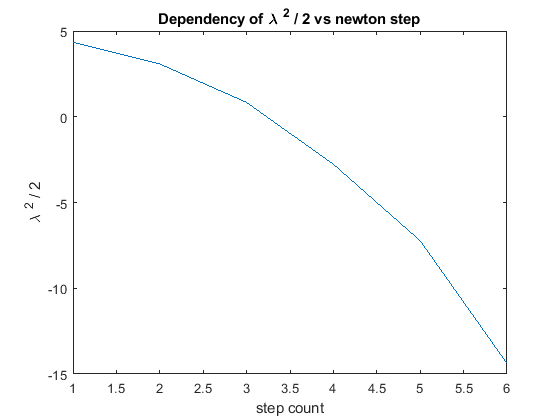
\includegraphics[width=\linewidth]{add_ex_plot.png}
	\caption{Dependency of $\lambda ^2 / 2$ vs. newton step}
\end{figure}


\end{document}